% Target: 8 pages with figures
\section{Least Response Time Load Balancing}
In this section we describe the role the load balancer plays in the context of our approach, how it is related to the underlying serverless platform, and the details of how it is implemented.

\subsection{Load Balancing Concepts}
While load balancing might at first appear as a rather simple problem, venturing outside cloud-centric scenarios, where resource homogeneity can be assumed, makes it much more complex of a challenge.
Since we feel the changes implied by resource heterogeneity are often only implicitly covered in literature, or an understanding of the problem is assumed, we believe that it is beneficial to describe it in more detail. This not only helps form a basis on which subsequent research can build, but also gives a lot of contextual information on how our approach relates to the underlying formal problem.

For our formulation of the load balancing problem we consider two types of resources: nodes, and network links. Nodes are the compute nodes in the cluster, and are characterized by the compute capabilities they possess and the function instances they host. Network links are characterized by their latency, and their bandwidth.
\begin{figure}
    \centering
    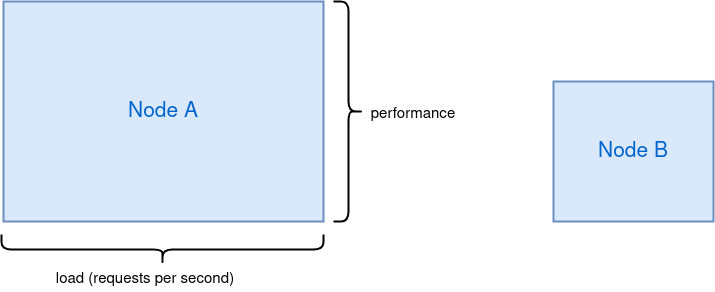
\includegraphics[width=12cm]{graphics/diagrams/load_balancer_squares.png}
    \caption{Rectangles representing a resource in our problem visualization}
    \label{fig:lb_squares_basic}
\end{figure}
To get a more intuitive understanding of the problem we developed a visualization, where resources are depicted as rectangles, and their dimensions correspond to their characterizing attributes. Figure \ref{fig:lb_squares_basic} shows an example of this. The width of the rectangle corresponds to the \textit{load} of the system, in our case measured in \gls{rps}, and the height corresponds to the performance, which since we are concerned about response times is the response time in milliseconds. One should note that, even though maybe counter intuitive, a greater height corresponds to higher performance, which in turn means \textit{lower} response times.
A core concept of this visualization is the capability of resources to \textit{stretch} or \textit{compress}. This means increasing or decreasing width or height of the resource, while doing the inverse to the other side. The condition is that the total area of the resource, i.e. the product of width and height, must be consistent throughout this process. This is effectively the way in which performance regression is modeled in this visualization, but one should note that this way only works under the condition that performance regression is linear with respect to the load. Luckily this is close to observed real world behaviour, %todo cite this
meaning that at least for understanding the underlying problem this visualization holds.
There are, however, limits to this stretching or compressing resources. From a visual perspective there is a bounding box around each resource, which cannot be exceeded in either height or width. This corresponds to the real world behaviour of workloads not getting faster beyond a certain point even if resources would be available on one side, and requests simply timing out once response times exceed a certain limit on the other.
\begin{figure}
    \centering
    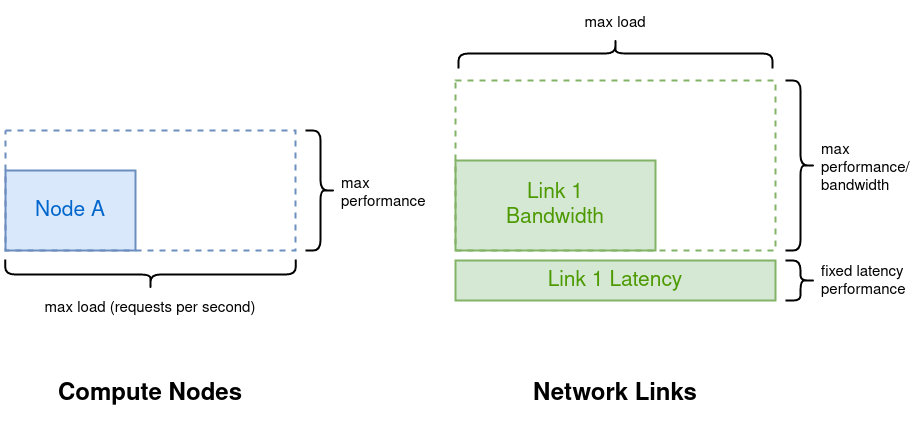
\includegraphics[width=14cm]{graphics/diagrams/lb_squares_real.png}
    \caption{Rectangles representing Node and Network Link resources, including their respective bounding boxes showing maximum load and performance capabilities}
    \label{fig:lb_squares_real}
\end{figure}
Network link resources work slightly differently, as they have a fixed component, dictated by the latency of the link, and a variable component set by the bandwidth. The variable component works as just described, while the static component is constant. Figure \ref{fig:lb_squares_real} shows the variable and static components along with their limits.

Resources can be conditionally linked. This maps the real world conditions of nodes being attached to the cluster via network links. Just like in actual clusters multiple nodes can be dependent on the same network link, and network links in turn can depend on another network link. 

\begin{figure}
    \centering
    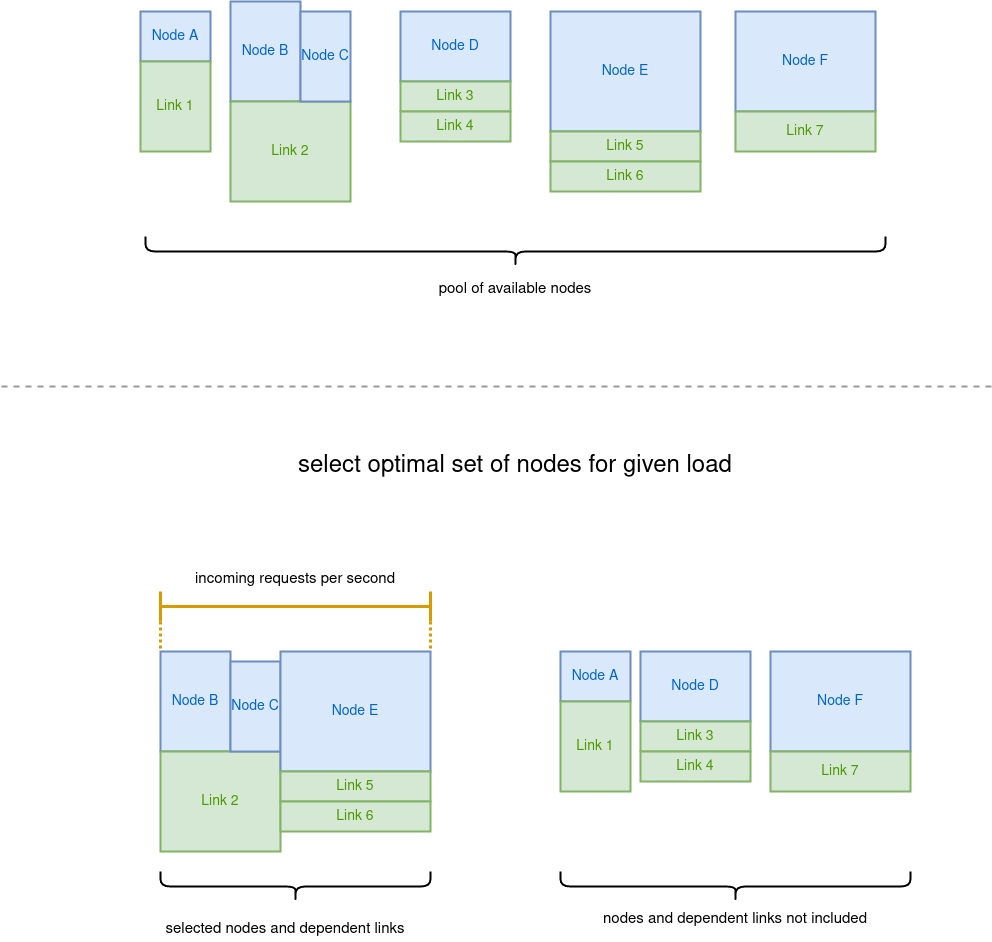
\includegraphics[width=14cm]{graphics/diagrams/lb_optimal_selection.png}
    \caption{Example visualization of an optimal selection of nodes, including their network links, for a given request load. Bounding boxes showing min/max load/performance, and fixed network latency performance parts are not displayed to keep the example simple.}
    \label{fig:lb_optimal_load}
\end{figure}

With this definition we can define the optimization problem an effective edge load balancer is trying to solve. The input to this problem is the given request load arriving from clients. In our visualization this corresponds to a set width. The objective is then to select nodes which when combined have the same width as the incoming client node, while at the same time maximizing the area of the nodes and network links selected. One needs to keep in mind that network links are not selected directly, but are implicitly included if selected nodes depend on them. Figure \ref{fig:lb_optimal_load} shows an example of such an optimal selection.

If the area is maximized in this optimization problem, response time is minimized, which is the goal a load balancer is trying to achieve.


While this visualization and problem is still relatively straightforward, there are other significant factors that we omitted until now:
\begin{enumerate}
    \item There are multiple functions, meaning that there are multiple "widths" or bins that need to be filled
    \item Functions share compute capabilities of nodes, meaning that performance regression, i.e. stretching and compression, needs to be considered over all functions running on a node
    \item Dependencies between network links and nodes aren't necessarily known
    \item Some network links necessarily handle traffic from outside the system, making performance regression assessment harder
    \item Actual performance profiles, i.e. dimensions, of nodes and functions aren't known
    \item Performance profiles, capabilities, client load, and function deployments change dynamically over time
\end{enumerate}

Considering these factors, load balancing in this context is a much higher-dimensional and thus more complex problem, where it is intuitively not clear whether an optimal solution is possible or if explicitly pursuing it in practise is even computationally feasible.


Since the true performance and regression characteristics of the nodes and network links are unknown, a load balancing solution needs to consider how this lack of information can be addressed. 
The simplest way to gather this information is by sending requests to nodes and observing response times. While this can yield insight into performance characteristics, these observations are merely a statistical sample, making them at least somewhat prone to misinterpretation. Especially when it comes to more complex behaviours such as functions sharing compute resources of nodes, or multiple nodes sharing network links.

Depending on the goals of the load balancer there is a risk/reward dynamic at play when it comes to sending requests to nodes in order to learn more about their performance characteristics. On one hand this can lead to "discovering" nodes that offer high performance and are able to handle a large number of requests, but on the other hand it could also lead to poor performance for those very requests in case network or compute capabilities are sub par.
There is no single correct answer to this dilemma, since the efficacy of any given solution would depend on the specific goals and tolerances of the application in question. In case \glspl{sla} exist that stipulate a certain response time for a minimum percentage of requests the risks might outweigh potential rewards, while an application that is somewhat tolerant to a fraction of requests being slow might experience a great performance uplift overall.
For our approach we consider \glspl{sla} to be out of scope, and therefore do not further address ways to address them. At the same time we want to point out that these are potentially relevant aspects for bringing serverless edge computing towards production readiness in the industry, and therefore highlight the areas where further study is needed.

\begin{figure}
    \centering
    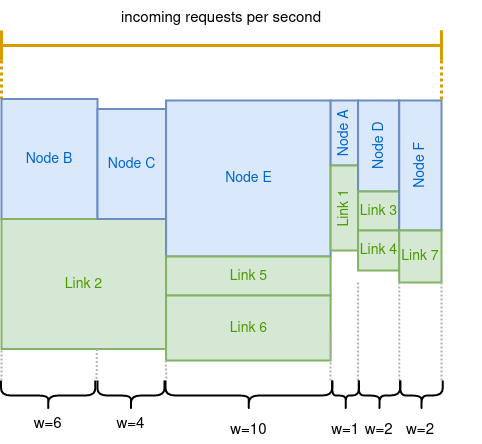
\includegraphics[width=10cm]{graphics/diagrams/lb_weights.png}
    \caption{Our approach as seen through the described visualization. All nodes are included in the "solution", and their load is determined by the load balancer assigning weights (w)}
    \label{fig:lb_weights}
\end{figure}

Considering the myriad of potentially complicating factors for load balancing, in particular if one were to attempt to directly model the problem algorithmically, we decided to take a comparatively simple approach for our load balancing method.
In our approach we base our load balancing decisions solely on the total response time as it is observed by the load balancer. This means that we do not differentiate between times incurred from \gls{fet} and the times incurred from the networking portion. In this way we treat the total response time as a \textit{black box metric} to the overall system.
Our approach is to always include every single node in the "solution" to selecting appropriate nodes for the given width. This means that over the long term our approach gathers information about every potential node for every function replica that gets requested.
The disadvantage of this approach is that it dispatches requests to nodes that would not be included in a mathematically optimal solution, meaning that is will never reach the optimal performance possible assuming perfect knowledge of the system.
To counteract the performance penalty of including all nodes in the solution we assign them weights based on the response time they achieve.
This allows the load balancer to strike a balance between gathering information about the performance of the nodes available to the cluster, and processing requests as fast as possible.
Figure \ref{fig:lb_weights} shows the view of our approach on the system as described in the visualization. Note that the networking portion is not present, as our approach only considers the total response time in relation to the node it was sent to. Our approach also views each function replica separately, meaning that joint performance degradation of co-located function replicas is not modeled explicitly, only implicitly via the degraded performance observable through total request response times on that node.

There are a number of important considerations about the practical realization of our approach, which we will discussed next.


\subsection{Implementation}
As was just outlined our approach uses the response time as a black box metric to get insights into the system, and thus make load balanced decisions based on that information.
Since the idea of using a black box metric alone does not constitute a concrete and testable approach we need to define the implementation details of how this concept can be applied in practise.

A well-known and simple implementation of this concept is the \textit{least response time} method of load balancing.
In this approach the server with the lowest average response time gets chosen whenever a request needs to be processed.
While this certainly works in general, and implicitly solves the proximity issue from Figure \ref{fig:efficient_path}, there are a few issues with this approach when it comes to serverless edge computing.
First, this approach can be problematic when it comes to co-located functions, as the load is not distributed among upstreams equally.
This leads to the fastest node being selected until its performance degrades enough for the next best node to be chosen.
Since there is no coordination that ensures some kind of balance, other functions that happen to be deployed on that node could experience severely hampered performance unexpectedly.
Second, this method does not take into account that the performance of nodes is, at least at first, unknown, and that it can change. A node that generally performs exceptionally well could be permanently excluded if at one point, for a spurious reason, performance was poor. A naive least response time load balancer would then likely rotate between a small handful of nodes that at one point performed well, effectively ignoring potentially better solutions.
These reasons point to the need of a more sophisticated approach than a naive implementation of least response time load balancing.

\subsubsection{Metrics Collection}
As explained, in our approach the metric used for load balancing decisions is the response time, specifically the time it takes between the load balancer forwarding the request to the selected upstream, and the load balancer receiving the response to the request.

Based on the response time data there are a number of performance metrics that could be calculated. Since our goal is to reduce the average total response time, we also chose the average response time as the key metric for load balancing decisions.
Depending on the requirements the load balancer needs to fulfill, other metrics could be used. A load balancer that is supposed to ensure a type of \gls{sla} might, for example, benefit from a percentile based metric instead.

In addition to effectively summarizing the performance of nodes, the metric needs to be time sensitive. Considering the performance of nodes can change over time, more recent values are more important as an indication of performance than those that lie farther back.
To address this, our approach makes use of a moving average with fixed window size.
We chose to use an exponential moving average since it has a number of advantages over more typical implementations.

Given the previous average value $\mathbf{\bar{r}_{0}}$, the most recent response time $\mathbf{r}$, the time passed since the last request $\mathbf{\Delta t}$, and the windows size $\mathbf{w}$, the new average value $\mathbf{\bar{r}_{1}}$ is

\[\bar{r}_{1} = (1 - e^{\frac{-\Delta t}{w}}) \cdot r + e^{\frac{-\Delta t}{w}} \cdot \bar{r}_{0}\]

The most significant advantage of this implementation over ones that use a buffer or a similar data structure, is precisely that complex data structures are not required. For each upstream only two values need to be recorded:
\begin{enumerate}
    \item The time the moving average was last updated
    \item The current value of the moving average itself
\end{enumerate}
While there are situations, where this can be less accurate, it is far easier to implement than buffer based solutions, since with these the required buffer size is unknown thus leading to frequent memory allocations and de-allocations.
Using an exponential moving average ensures minimal memory consumption, while at the same time being easy to understand and implement.

\subsubsection{Choosing Upstreams}
With the metrics collected what remains is deciding on upstreams based on those values. As previously outlined, naively choosing the upstream with the lowest average response time is potentially problematic.
For this reason our approach uses weighted round robin to decide which upstream should service a given request, where the response time metrics determine the weight assigned to each upstream.

The decision how exactly this weighted round robin gets implemented is surprisingly important, since the load balancing decisions affect the accuracy and volume of performance data gathered on each node, thus creating a feedback cycle that can, depending on the situation, lead to sub optimal performance.
For our approach we decided to use the same method employed by NGINX\cite{nginx}, a popular web-server and request proxy.
We chose this approach after experimenting with other solutions, and analyzing their performance profiles and characteristics with regard to the unique challenges posed by serverless edge computing environments.
Compared to other approaches is has the advantage of being deterministic, leading to all nodes being chosen eventually, which gives the load balancer sufficient data to make informed decisions, while at the same time distributing traffic in a mixed fashion between upstreams of different weights.
The evaluation methodology and experiment results of these experiments can be found alongside the general evaluation in the subsequent chapters.

\begin{algorithm}
  \KwIn{Set of available nodes $n_{0},n_{1},n_{...} \in N$}
  \KwIn{Weights for each of the nodes $w_{n_{0}}, w_{n_{1}}, ... \in W$}
  \KwIn{Current counter value for each node. $c_{n_{0}}, c_{n_{0}}, ... \in C$}
  \KwOut{The node the next request should go to}
    \For{$n \in N$}
    {
        $c_{n} \leftarrow c_{n} + w_{n}$ \Comment{add node weight to its counter}
    }
    $\text{selectedNode} \leftarrow n: c_{n} = max\{c: c \in C\}$ \Comment{select node with highest counter value}\\
    $c_{\text{selectedNode}} \leftarrow c_{\text{selectedNode}} - \sum_{w \in W}w$\\
    
  \Return{selectedNode}

  \caption{Smooth Weighted Round Robin}
  \label{alg:smooth-wrr}
\end{algorithm}
%todo: maybe rework this to be a bit more elegant
% currently a bit too much of a mashup between, math, set theory, code

\begin{table}[]
\centering
\begin{tabular}{llll}
Node          & \textbf{A}                & \textbf{B}                & \textbf{C}                \\
Weight        & \textbf{4}                & \textbf{2}                & \textbf{1}                \\ \hline
Iteration \#1 & \cellcolor[HTML]{FFCE93}4 & 2                         & 1                         \\
              & -3                        & 2                         & 1                         \\ \hline
Iteration \#2 & 1                         & \cellcolor[HTML]{FFCE93}4 & 2                         \\
              & 1                         & -3                        & 2                         \\ \hline
Iteration \#3 & \cellcolor[HTML]{FFCE93}5 & -1                        & 3                         \\
              & -2                        & -1                        & 3                         \\ \hline
Iteration \#4 & 2                         & 1                         & \cellcolor[HTML]{FFCE93}4 \\
              & 2                         & 1                         & -3                        \\ \hline
Iteration \#5 & \cellcolor[HTML]{FFCE93}6 & 3                         & -2                        \\
              & -1                        & 3                         & -2                        \\ \hline
Iteration \#6 & 3                         & \cellcolor[HTML]{FFCE93}5 & -1                        \\
              & 3                         & -2                        & -1                        \\ \hline
Iteration \#7 & \cellcolor[HTML]{FFCE93}7 & 0                         & 0                         \\
              & 0                         & 0                         & 0                        
\end{tabular}
\caption{An example of weighted round robin iteration results when using Algorithm \ref{alg:smooth-wrr} as we do in our approach. Colored cells indicate the selected node at the iteration.}
\label{tab:smooth-wrr-demo}
\end{table}

Algorithm \ref{alg:smooth-wrr} shows a pseudo-code implementation of our weighted round robin component using the approach also used in the NGINX source code \cite{nginx-wrr}.
Table \ref{tab:smooth-wrr-demo} shows how this implementation of weighted round robin distributes requests between upstreams of different weights. Note that the proportions between the weights are considered when choosing upstreams without using a fixed ordering based on weight, meaning that choices of upstreams with lower weights are interleaved between choices of upstreams with higher weights. %todo rewrite this. It's super unclear what is meant by this.

The only part of our load balancing approach that is not yet described is how the average response time recorded is mapped to the weight used by our weighted round robin implementation.
There are a number of ways in which values like this can get mapped to weights.
There is, unfortunately, no single correct answer since the lack of precise information on the state and performance of nodes and the network prevents us from reliably making globally optimal load balancing decisions.
There are two factors that determine how response times are mapped to weights:
\begin{enumerate}
    \item The weight range response times should be mapped to
    \item The function by which they are mapped to these weights
\end{enumerate}

In our approach we chose to use a fixed range of weights, since this makes sure every upstream is assigned at least a fixed fraction of traffic.
This guarantees that the response times of all upstreams are sampled eventually, preventing a situation where a significant change in the performance of an upstream goes unnoticed forever.
The weight of each upstream is determined by it's average response time in the last value and calculated using the following formula:

Let $\mathbf{\bar{r} \in R}$ be the set of response time averages, $\mathbf{w_{\text{min}}}$ the minimum weight, and $\mathbf{w_{\text{max}}}$ the maximum weight. Then the weight for each response time average $\mathbf{w(\bar{r})}$ is defined as

\[ w(\bar{r}) = max\{w_{\text{min}}, \frac{w_{\text{max}}}{(\frac{\bar{r}}{min\{\bar{r}: \bar{r} \in R\}})^{s}}\} \]

where $\mathbf{s > 0}$ is a chosen scaling factor.

% \[ \text{Let } \bar{r} \in R \text{ be the set of response time averages, and }\]
% \[ w_{\text{min}} \text{ the minimum weight, } w_{\text{max}} \text{ the maximum weight, then}\]
% \[ \text{the weight for each response time average } w(\bar{r})\text{ is defined as}\]

% \[ \text{where } s > 0\text{ is a chosen scaling factor }\]

The scaling factor determines how weights correlate to response time. A scaling factor of 1 means that there is a linear relationship between the average performance and the weight.
Figure \ref{fig:weight_mapping_example} shows the effect different scaling factors have on weight mappings in the weight range of 1-10. Both continuous and integer values are shown, since it depends on the weighted round robin implementation which of the two can be used.
Based on grid-search experiments we chose a weight range of 1-25, and a scaling factor of 2, although we stress that there is no one optimal parameter choice for all circumstances.
The experiments that determined this choice will be described in detail in subsequent chapters.

% idea: factor (i.e. deciding on linearity) depends on how strong the link between performance and capacity is. i.e. if strong performance means high capacity, we can assign super high relative weights. Is this even important? Since on paper overload etc. should eventually lead to a balance being achieved, no?
% idea: spread (i.e. size of weight range) depends on how dynamic the system is and how high we value information gain, since high spread -> more optimal in static condition. low spread -> discovers changes faster in dynamic conditions.

\begin{figure}
    \centering
    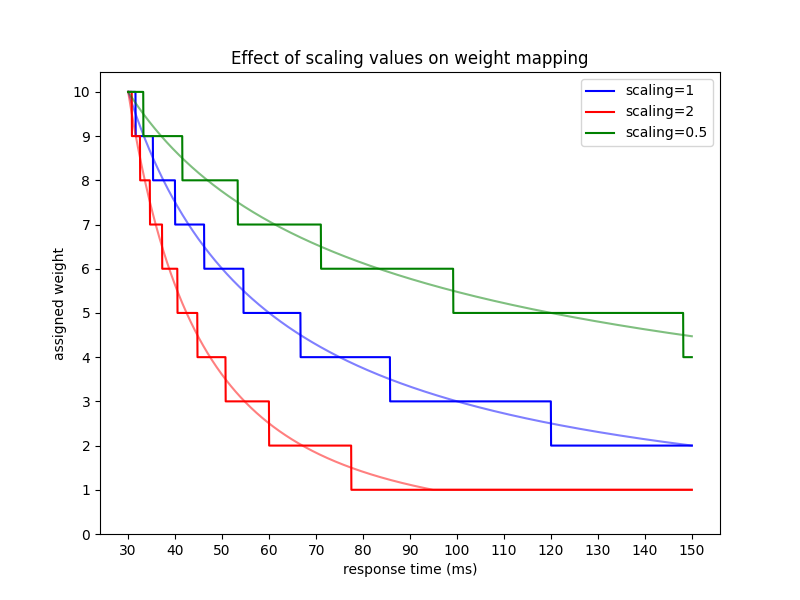
\includegraphics[width=10cm]{graphics/graphs/weight_mapping_scaling_example.png}
    \caption{Plot showing the effects of different scaling factors on how response time averages are mapped to weights.}
    \label{fig:weight_mapping_example}
\end{figure}


\subsubsection{Framework Integration}
In our approach the load balancers are assumed to be integrated into the serverless framework.
This means that load balancers are notified of changes to function replicas, meaning that they are always aware which functions exist, and which exact replicas are available for each function.
From a practical perspective this is simple to achieve in a production implementation as serverless frameworks already provide this information in some way, and the underlying technologies, typically some kind of container orchestration, also have means to retrieve the necessary data.

Apart from the available functions and their respective replicas, new load balancer instances are initialized with response time values and weights of already running load balancer instances nearby.
While the load balancer still needs to adapt its weights based on its specific client load and position in the network, this initial pre-loading of values allows it to converge on a stable configuration faster, thus resulting in quicker performance gains.

